% Options for packages loaded elsewhere
\PassOptionsToPackage{unicode}{hyperref}
\PassOptionsToPackage{hyphens}{url}
%
\documentclass[
  12pt,
  a4paperpaper,
]{book}

\usepackage{amsmath,amssymb}
\usepackage[]{gfsartemisia}
\usepackage{setspace}
\usepackage{iftex}
\ifPDFTeX
  \usepackage[T1]{fontenc}
  \usepackage[utf8]{inputenc}
  \usepackage{textcomp} % provide euro and other symbols
\else % if luatex or xetex
  \usepackage{unicode-math}
  \defaultfontfeatures{Scale=MatchLowercase}
  \defaultfontfeatures[\rmfamily]{Ligatures=TeX,Scale=1}
\fi
% Use upquote if available, for straight quotes in verbatim environments
\IfFileExists{upquote.sty}{\usepackage{upquote}}{}
\IfFileExists{microtype.sty}{% use microtype if available
  \usepackage[]{microtype}
  \UseMicrotypeSet[protrusion]{basicmath} % disable protrusion for tt fonts
}{}
\usepackage{xcolor}
\usepackage[heightrounded,margin = 25mm,headheight = 5cm,showframe =
true]{geometry}
\setlength{\emergencystretch}{3em} % prevent overfull lines
\setcounter{secnumdepth}{3}
% Make \paragraph and \subparagraph free-standing
\ifx\paragraph\undefined\else
  \let\oldparagraph\paragraph
  \renewcommand{\paragraph}[1]{\oldparagraph{#1}\mbox{}}
\fi
\ifx\subparagraph\undefined\else
  \let\oldsubparagraph\subparagraph
  \renewcommand{\subparagraph}[1]{\oldsubparagraph{#1}\mbox{}}
\fi
\pagestyle{headings}

\usepackage{color}
\usepackage{fancyvrb}
\newcommand{\VerbBar}{|}
\newcommand{\VERB}{\Verb[commandchars=\\\{\}]}
\DefineVerbatimEnvironment{Highlighting}{Verbatim}{commandchars=\\\{\}}
% Add ',fontsize=\small' for more characters per line
\usepackage{framed}
\definecolor{shadecolor}{RGB}{253,246,227}
\newenvironment{Shaded}{\begin{snugshade}}{\end{snugshade}}
\newcommand{\AlertTok}[1]{\textcolor[rgb]{0.83,0.21,0.51}{\textbf{#1}}}
\newcommand{\AnnotationTok}[1]{\textcolor[rgb]{0.15,0.55,0.82}{#1}}
\newcommand{\AttributeTok}[1]{\textcolor[rgb]{0.15,0.55,0.82}{#1}}
\newcommand{\BaseNTok}[1]{\textcolor[rgb]{0.16,0.63,0.60}{#1}}
\newcommand{\BuiltInTok}[1]{\textcolor[rgb]{0.80,0.29,0.09}{#1}}
\newcommand{\CharTok}[1]{\textcolor[rgb]{0.16,0.63,0.60}{#1}}
\newcommand{\CommentTok}[1]{\textcolor[rgb]{0.58,0.63,0.63}{\textit{#1}}}
\newcommand{\CommentVarTok}[1]{\textcolor[rgb]{0.16,0.63,0.60}{#1}}
\newcommand{\ConstantTok}[1]{\textcolor[rgb]{0.16,0.63,0.60}{\textbf{#1}}}
\newcommand{\ControlFlowTok}[1]{\textcolor[rgb]{0.52,0.60,0.00}{\textbf{#1}}}
\newcommand{\DataTypeTok}[1]{\textcolor[rgb]{0.71,0.54,0.00}{\textbf{#1}}}
\newcommand{\DecValTok}[1]{\textcolor[rgb]{0.16,0.63,0.60}{#1}}
\newcommand{\DocumentationTok}[1]{\textcolor[rgb]{0.86,0.20,0.18}{#1}}
\newcommand{\ErrorTok}[1]{\textcolor[rgb]{0.86,0.20,0.18}{\underline{#1}}}
\newcommand{\ExtensionTok}[1]{\textcolor[rgb]{0.15,0.55,0.82}{\textbf{#1}}}
\newcommand{\FloatTok}[1]{\textcolor[rgb]{0.16,0.63,0.60}{#1}}
\newcommand{\FunctionTok}[1]{\textcolor[rgb]{0.15,0.55,0.82}{#1}}
\newcommand{\ImportTok}[1]{\textcolor[rgb]{0.16,0.63,0.60}{#1}}
\newcommand{\InformationTok}[1]{\textcolor[rgb]{0.71,0.54,0.00}{#1}}
\newcommand{\KeywordTok}[1]{\textcolor[rgb]{0.52,0.60,0.00}{\textbf{#1}}}
\newcommand{\NormalTok}[1]{\textcolor[rgb]{0.40,0.48,0.51}{#1}}
\newcommand{\OperatorTok}[1]{\textcolor[rgb]{0.52,0.60,0.00}{#1}}
\newcommand{\OtherTok}[1]{\textcolor[rgb]{0.52,0.60,0.00}{#1}}
\newcommand{\PreprocessorTok}[1]{\textcolor[rgb]{0.80,0.29,0.09}{#1}}
\newcommand{\RegionMarkerTok}[1]{\textcolor[rgb]{0.15,0.55,0.82}{\colorbox[rgb]{0.93,0.91,0.84}{#1}}}
\newcommand{\SpecialCharTok}[1]{\textcolor[rgb]{0.86,0.20,0.18}{#1}}
\newcommand{\SpecialStringTok}[1]{\textcolor[rgb]{0.86,0.20,0.18}{#1}}
\newcommand{\StringTok}[1]{\textcolor[rgb]{0.16,0.63,0.60}{#1}}
\newcommand{\VariableTok}[1]{\textcolor[rgb]{0.15,0.55,0.82}{#1}}
\newcommand{\VerbatimStringTok}[1]{\textcolor[rgb]{0.16,0.63,0.60}{#1}}
\newcommand{\WarningTok}[1]{\textcolor[rgb]{0.80,0.29,0.09}{#1}}

\providecommand{\tightlist}{%
  \setlength{\itemsep}{0pt}\setlength{\parskip}{0pt}}\usepackage{longtable,booktabs,array}
\usepackage{calc} % for calculating minipage widths
% Correct order of tables after \paragraph or \subparagraph
\usepackage{etoolbox}
\makeatletter
\patchcmd\longtable{\par}{\if@noskipsec\mbox{}\fi\par}{}{}
\makeatother
% Allow footnotes in longtable head/foot
\IfFileExists{footnotehyper.sty}{\usepackage{footnotehyper}}{\usepackage{footnote}}
\makesavenoteenv{longtable}
\usepackage{graphicx}
\makeatletter
\def\maxwidth{\ifdim\Gin@nat@width>\linewidth\linewidth\else\Gin@nat@width\fi}
\def\maxheight{\ifdim\Gin@nat@height>\textheight\textheight\else\Gin@nat@height\fi}
\makeatother
% Scale images if necessary, so that they will not overflow the page
% margins by default, and it is still possible to overwrite the defaults
% using explicit options in \includegraphics[width, height, ...]{}
\setkeys{Gin}{width=\maxwidth,height=\maxheight,keepaspectratio}
% Set default figure placement to htbp
\makeatletter
\def\fps@figure{htbp}
\makeatother
\newlength{\cslhangindent}
\setlength{\cslhangindent}{1.5em}
\newlength{\csllabelwidth}
\setlength{\csllabelwidth}{3em}
\newlength{\cslentryspacingunit} % times entry-spacing
\setlength{\cslentryspacingunit}{\parskip}
\newenvironment{CSLReferences}[2] % #1 hanging-ident, #2 entry spacing
 {% don't indent paragraphs
  \setlength{\parindent}{0pt}
  % turn on hanging indent if param 1 is 1
  \ifodd #1
  \let\oldpar\par
  \def\par{\hangindent=\cslhangindent\oldpar}
  \fi
  % set entry spacing
  \setlength{\parskip}{#2\cslentryspacingunit}
 }%
 {}
\usepackage{calc}
\newcommand{\CSLBlock}[1]{#1\hfill\break}
\newcommand{\CSLLeftMargin}[1]{\parbox[t]{\csllabelwidth}{#1}}
\newcommand{\CSLRightInline}[1]{\parbox[t]{\linewidth - \csllabelwidth}{#1}\break}
\newcommand{\CSLIndent}[1]{\hspace{\cslhangindent}#1}

% Load packages
\usepackage{titling}
\usepackage{authoraftertitle}
\usepackage{setspace}
% \usepackage{titlesec}
% \usepackage[pagestyles]{titlesec}

% Set space between paragraphs and indent
% \usepackage[skip=10pt plus1pt, indent=20pt]{parskip}



% 
% \usepackage[skip=10pt plus1pt]{parskip}
% \parindent = 20pt





% \oneandahalfspacing

% \titleformat
% {\chapter} % command
% [display] % shape
% {\bfseries\Large\itshape} % format
% {Story No. \ \thechapter} % label
% {0.5ex} % sep
% {
%     \rule{\textwidth}{1pt}
%     \vspace{1ex}
%     \centering
% } % before-code
% [
% \vspace{-0.5ex}%
% \rule{\textwidth}{0.3pt}
% ] % after-code

% \titleformat{\chapter}%
%   {\normalfont\bfseries\Huge}{\thechapter.}{10pt}{}
% \newpagestyle{mystyle}{
%   \sethead[][\thechapter.\enspace\chaptertitle][]{}{\thesection~\sectiontitle}{}
% \setfoot{}{\thepage}{}}
% 




\setlength{\droptitle}{-3cm}
\preauthor{
  \begin{center}
  
\includegraphics[width=5in,height=4in]{cover.png}\\ % cover figure
  \Large
  \vspace{10mm}
}
\postauthor{
  \end{center}
}
\predate{
  \begin{center}
  Collège International des Scicences Territoriales \\ 
  Encadré par Hugues Pécout - Ingénieur de recherche, géomaticien\\
  \vspace{5mm}
  Master Carthagéo\\
  \vspace{5mm}
}
\postdate{
  \vspace{10mm}
  \\
  
\includegraphics[width=4in,height=1in]{figures/logos/logos3.jpg}\\
  % 
\includegraphics[width=1.5in,height=1.5in]{figures/logos/logos.jpg}\\
  \end{center}
  \newpage
  \mbox{}
  \vfill
  % Cover page\\
  % \emph{Beckwithia glacialis} on Snøhetta.
 }
\makeatletter
\makeatother
\makeatletter
\@ifpackageloaded{bookmark}{}{\usepackage{bookmark}}
\makeatother
\makeatletter
\@ifpackageloaded{caption}{}{\usepackage{caption}}
\AtBeginDocument{%
\ifdefined\contentsname
  \renewcommand*\contentsname{Table of contents}
\else
  \newcommand\contentsname{Table of contents}
\fi
\ifdefined\listfigurename
  \renewcommand*\listfigurename{List of Figures}
\else
  \newcommand\listfigurename{List of Figures}
\fi
\ifdefined\listtablename
  \renewcommand*\listtablename{List of Tables}
\else
  \newcommand\listtablename{List of Tables}
\fi
\ifdefined\figurename
  \renewcommand*\figurename{Figure}
\else
  \newcommand\figurename{Figure}
\fi
\ifdefined\tablename
  \renewcommand*\tablename{Table}
\else
  \newcommand\tablename{Table}
\fi
}
\@ifpackageloaded{float}{}{\usepackage{float}}
\floatstyle{ruled}
\@ifundefined{c@chapter}{\newfloat{codelisting}{h}{lop}}{\newfloat{codelisting}{h}{lop}[chapter]}
\floatname{codelisting}{Listing}
\newcommand*\listoflistings{\listof{codelisting}{List of Listings}}
\makeatother
\makeatletter
\@ifpackageloaded{caption}{}{\usepackage{caption}}
\@ifpackageloaded{subcaption}{}{\usepackage{subcaption}}
\makeatother
\makeatletter
\makeatother
\ifLuaTeX
  \usepackage{selnolig}  % disable illegal ligatures
\fi
\IfFileExists{bookmark.sty}{\usepackage{bookmark}}{\usepackage{hyperref}}
\IfFileExists{xurl.sty}{\usepackage{xurl}}{} % add URL line breaks if available
\urlstyle{same} % disable monospaced font for URLs
\hypersetup{
  pdftitle={Gestion d'une base de données qualitative et géometrique},
  pdfauthor={Elina Marveaux},
  hidelinks,
  pdfcreator={LaTeX via pandoc}}

\title{Gestion d'une base de données qualitative et géometrique}
\author{Elina Marveaux}
\date{12 Juin 2022}

\begin{document}
\frontmatter
\maketitle
Résumé du stage (dont le sujet) en 10 lignes en français et en anglais. Informatif et concis, ce résumé doit refléter l'esprit du document, définir les buts et les méthodes, les résultats et les conclusions. Il se présente sous la forme d'un paragraphe unique, sans alinéa.

\renewcommand*\contentsname{Table des matières}
{
\setcounter{tocdepth}{2}
\tableofcontents
}
\setstretch{1.5}
\mainmatter
\bookmarksetup{startatroot}

\hypertarget{introduction}{%
\chapter*{Introduction}\label{introduction}}
\addcontentsline{toc}{chapter}{Introduction}

Elle doit mentionner : les objectifs, les lieux d'étude, l'intérêt du
projet : pour un public particulier ? Une nouvelle méthodologie ? Une
monographie sur un espace donné ? Durée. Un rapport orienté « recherche
» développera la problématique qui sous-tend le questionnement de
recherche et formulera, le cas échéant, les hypothèses de travail.

\begin{center}\rule{0.5\linewidth}{0.5pt}\end{center}

This is a Quarto book.

To learn more about Quarto books visit
\url{https://quarto.org/docs/books}.

\begin{Shaded}
\begin{Highlighting}[numbers=left,,]
\DecValTok{1} \SpecialCharTok{+} \DecValTok{1}
\end{Highlighting}
\end{Shaded}

\begin{verbatim}
[1] 2
\end{verbatim}

\begin{figure}

{\centering 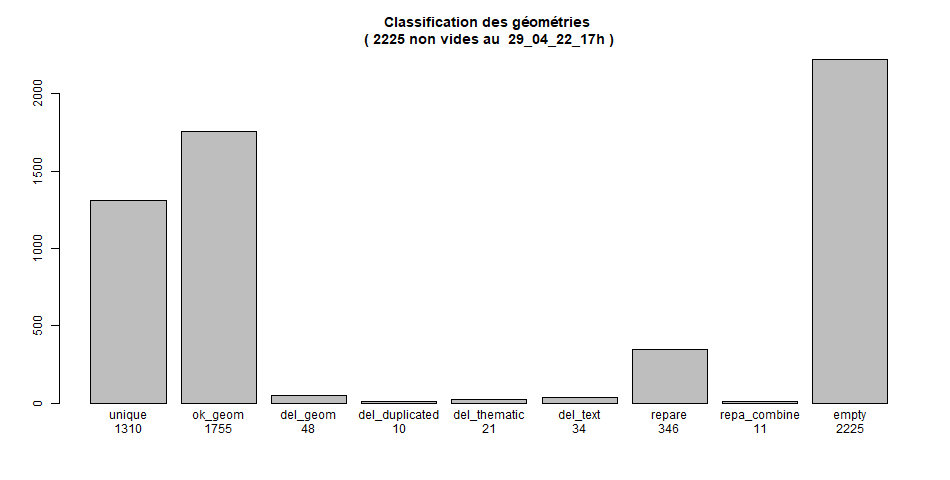
\includegraphics{./figures/bar_classify_Del_29_04_22_17h.png}

}

\caption{Chart Bar des NAS}

\end{figure}

\bookmarksetup{startatroot}

\hypertarget{notes-rendez-vous-antonine}{%
\chapter*{Notes rendez-vous Antonine}\label{notes-rendez-vous-antonine}}
\addcontentsline{toc}{chapter}{Notes rendez-vous Antonine}

Dimension politique des visualisation à mettre en avant

\hypertarget{les-visualisations}{%
\section*{Les visualisations}\label{les-visualisations}}
\addcontentsline{toc}{section}{Les visualisations}

Faire la différences entres les visualisations des polygone sen internes
pour leur diagnostique et la présentation des ``problèmes'' et la
représentation finale, les cartographies qui doivent être finie et
présentées comme résultat et non pas comme exploration.\\
Les deux modes de représentations font appels à des enjeux différents
(ainsi que des publiques, objectifs)

\hypertarget{muxe9thodologie}{%
\section*{Méthodologie}\label{muxe9thodologie}}
\addcontentsline{toc}{section}{Méthodologie}

\begin{itemize}
\tightlist
\item
  Décrire la méthodologie
\item
  Quelle est la qualité de l'information :
\item
  Qualité du point de vue de la géomatique
\item
  Quels biais introduits dans les enquêtes ``habituelles'' ou en tout
  cas celle précédent celle-ci (eurobroadmap)
\item
  Quel biais introduits par la méthodologie actuelle, quel enjeux vis à
  vis du choix de l'outil
\item
  Comment sont identifiés/détectés les problèmes dans la BD et BDG,
  quelles propositions sont avancées , lesquelles sont mises en place et
  comment trancher ? **proposer une chaîne de traitement sous forme
  d'image''
\item
  Voir Lena Sanders : modèle LOgit pour explorer la significativité ou
  non du univ\_field
\item
  Quelle pondération de polygones lorsqu'ils se superposent, lorsqu'ils
  n'ont pas la même taille mais décrivent des ensembles similaires
  (pays) ou lorsqu'il sont multi-polygones donc séparés et parfois se
  recouvrent
\item
  Comment analyser les aires disjointes ou emboîtées ?
\end{itemize}

\hypertarget{analyse-du-besoin-en-amont}{%
\section*{Analyse du besoin en amont
?}\label{analyse-du-besoin-en-amont}}
\addcontentsline{toc}{section}{Analyse du besoin en amont ?}

\hypertarget{livrables}{%
\section*{Livrables}\label{livrables}}
\addcontentsline{toc}{section}{Livrables}

\begin{itemize}
\tightlist
\item
  Quels sont les produits à réalisés et à qui s'adressent-ils ?
\item
  Priorité sur les \textbf{géométries} et leur enjeux :
\item
  plusieurs dessins sont autorisées
\item
  plusieurs modes de saisi sont possibles chacun avec leur biais
\item
  Plusieurs problèmes en découlent
\item
  Base de donnée Géo et Respondent avec documents de présentation
\item
  explorations de la BDG :
\item
  Visualisations exploratoires et travail de représentation pour le
  diagnostic (explorer les chorèmes pour proposer une typologie des
  polygones et relations rencontrées dans la BDG)
\item
  Visualisations finales / exploratoires en tant de résultats de
  l'exploration : on parle de représentations visant à proposer
  certaines interprétations des résultats (sous formes de prototypes car
  la valorisation finale est attendue en dehors du cadre du stage)
\end{itemize}

\hypertarget{git}{%
\section*{GIT}\label{git}}
\addcontentsline{toc}{section}{GIT}

\begin{itemize}
\tightlist
\item
  expliquer l'intérêt de l'outil
\item
  Faire la différence entre 'usage généraliste de l'outil et l'usage
  qu'on en fait en interne (dans le care du stage notamment)
\item
  Expliquer pourquoi une page web et quel est l'intérêt (éventuellement
  pour mettre à disposition des résultats du stage et la présentation du
  mémoire ar exemple)
\end{itemize}

\hypertarget{gestion-de-projet-workshop}{%
\section*{Gestion de projet /
Workshop}\label{gestion-de-projet-workshop}}
\addcontentsline{toc}{section}{Gestion de projet / Workshop}

Ici discuter des apports du stage dans le domaine de la gestion de
projet et de la mise en place d'un workshop. - Dans quelle mesure
suis-je force de proposition - Quel suivi, même informel est mis ou
ai-je mis en place ? Finalement le suivi est assez souple, je suis libre
de faire ce que je veux mais le cadre est bien posé et les objectifs
déterminés. Par exemple, j'ai été accompagnée dans la découverte de la
BD e des premiers scripts exploratoires, j'ai eu comme objectif de
réaliser un document de présentation de cette base de donnée et des
traitements qui y ont été réalisés pour la rendre propre ou qui peuvent
être réalisés dessus en guise d'exploration. J'ai le champ libre pour la
réalisation de ce document concernant à la fois les outils que j'utilise
et ce que j'y met. Je reste encadrée lorsque j'ai des questions et ait
besoin d'être recadrée.

\begin{itemize}
\tightlist
\item
  Mettre ne avant l'informel : les formations et les autres projets/
  présentations auxquelles j'ai été invitées à participer
\item
  Parler des compétences acquises en matière de logiciels/ technique
  (quarto, redaction latex/yaml, regex, git )
\end{itemize}

\hypertarget{la-forme-du-muxe9moire}{%
\section*{La forme du mémoire}\label{la-forme-du-muxe9moire}}
\addcontentsline{toc}{section}{La forme du mémoire}

\begin{itemize}
\item
  utiliser souvent les illustrations et les graphiques, notamment pour
  les chaines de traitement et l'organisation. il est important que le
  mémoire reste lisible et très rapidement compréhensible.
\item
  \textbf{Etat de l'art} : Surtout un état de l'existant notamment en
  matière d'outils et de méthodologie. Le stage reste un stage
  ingénieur, et non pas de recherche. Il faut mettre en avant ce qui a
  déjà été produit en terme technique (exemple : si je rencontre un
  problème, la solution existe probablement déjà, il faut alors que je
  fasse été de cette ou ces solutions et que je discute de ce que j'en
  fait, comment je l'adapte à mon travail etc
\item
  Deux options pour le plan :
\item
  Classique : 3 parties reprenant chacune tous les objectifs / sous
  projets

  \begin{itemize}
  \tightlist
  \item
    Contexte (structure, projet, enjeux du projet, comment le stage
    s'insère dans le projet, quels acteurs sont rencontrés et quels sont
    leurs rôles)
  \item
    Méthodologie mise en place
  \item
    Résultats avec mise en perspective, retour sur le travail effectué
  \end{itemize}
\item
  ou alors Une partie par projet / Objectif reprenant chacune les
  parties précédemment décrites

  \begin{itemize}
  \tightlist
  \item
    1 : exploration BDR : Contexte/méthodologie/résultats
  \item
    2 : Exploration des géométries Contexte/méthodologie/résultats
  \end{itemize}
\item
  Bien mettre en avant ce que j'ai découvert, ce que j'ai
  \textbf{proposé} les difficultés rencontrées et les problèmes soulevés
  même s'ils n'ont pas été résolus
\item
  \textbf{OBJECTIFS} : reproductibilité, analyse, mise à disposition des
  données (et proposition d'exploitation de ces données
\end{itemize}

\bookmarksetup{startatroot}

\hypertarget{contexte}{%
\chapter{Contexte}\label{contexte}}

\begin{quote}
Contexte (structure, projet, enjeux du projet, comment le stage s'insère
dans le projet, quels acteurs sont rencontrés et quels sont leurs rôles)
\end{quote}

\hypertarget{le-c.i.s.t}{%
\section{Le C.I.S.T}\label{le-c.i.s.t}}

Présentation de la Fédération de recherche, de sa structuration et des
axes, en précisan qu'a terme je travaillerai ussi sur cers projets bien
qu'ils ne fassent pas parti du stage.

\hypertarget{imageun-et-lanr---dfg}{%
\subsection{IMAGEUN et l'ANR - DFG}\label{imageun-et-lanr---dfg}}

Présenter l'objectif principal du projet, les workshops et les acteurs.
En venir au \textbf{Workshop - students} surlequel je travaille dans le
cadre du stage et détailler mon rôle, expliquer la Base de donnée ce qui
a été mis en place avant mon arrivée (de quoi je pars) dan les grandes
lignes sans entrer dans les problèmes etc\ldots{}

Présenter ensuite la collecte et la base de donnée générale : -
temporalité effectifs objectifs réalisés ou non

\hypertarget{eurobroadmap-et-glocal-map}{%
\section{EuroBroadMap et Glocal Map}\label{eurobroadmap-et-glocal-map}}

Les résultats Europe sont très normées, voir prévisibles, tandis que
d'autres pays adoptent un regard plus critique vis à vis de l'Europe. -
Chine mode, luxe, sp Afrique : Tunisie et Sénégal : crique sur le
racisme / inégalité / colonialisme Brésil :

\hypertarget{echuxe9ances}{%
\section{Echéances}\label{echuxe9ances}}

\begin{itemize}
\tightlist
\item
  15 Juin - \textbf{50 ans de l'ANR DFG} : \emph{Production d'une
  ``image'' comprenant des cartes lissées des premiers résultats pour la
  France et l'allemagne ainsi que des nuages de mots décrivant l'Europe}
\item
  20/24 Juin - \textbf{Ecole d'Ete} : \emph{Pas directent en lien avec
  le stage mais plutot avec les missions de la Fédération de recherche}
\item
  23/26 Juin - \textbf{Tachkent} : \emph{Préparation des données issues
  des réponses turques pour la doctorante travaillant sur le projet. Il
  s'agissait pour elle de présenter ces résultts à une conférence avec
  le partenaire Turc.}

  \begin{itemize}
  \tightlist
  \item
    Typologie des polygones
  \item
    Cartographie de ces polygones
  \item
    Nettoyage de BD et réalisation d'un dictionnaire réduit à l'usage du
    partenaire
  \item
    Production de graphiques et résultats statistiques préliminaires
  \end{itemize}
\item
  \textbf{30 Juin : ARRET DE LA DIFFUSION DU QUESTIONNAIRE}
\item
  18/22 Juillet - \textbf{UGI - Congrès Centenaire de l'Union
  Géographique Internationale} : \emph{Préparation des données propres
  et prete à etre exploitées}

  \begin{itemize}
  \tightlist
  \item
    Typoogie des polygones restants
  \item
    Cartographie pour chaque pays / ville / université
  \item
    Graphiques pour chaque pays / ville / université
  \item
    \ldots{}
  \end{itemize}
\item
  18 Septembre - \textbf{JIG Journée des jeunes chercheurs de l'institut
  de géographie} : \emph{Réalisation d'un poster}
\end{itemize}

\hypertarget{objectifs}{%
\section{Objectifs}\label{objectifs}}

Livrer une base de donnée et des traitements s'inscrivant dans la
reproductibilité, mais l'arrivée de la base de donnée finale s'étant
faite tardivement nous avons plutôt opté pour une chaîne de traitement
propre, dirigée vers les besoins immédiats des acteurs (Tachkent, UGI,
mémoire). la mise en pacquage se fera certainement dans un deuxième
temps, d'autant plus que le contrat se poursuit au delà du stage pour
ces missions là (ainsi que pour de la valorisation).

Il était donc question de mettre en place des traitements de géomatiques
(SIG géotraitements des géométries et données spatialisées) ainsi que
des traitements textuels (cordonner notamment la traduction). Il a fallu
dans un premier temps me familiariser avec la base de donnée avant de
détecter les problèmes et d'en proposer les corrections.

Je suis partie d'une base de programmes ayant servis aux premières
explorations (graphiques statistiques généraux sur les taux de réponses
et premières visualisation des géométries). Mon travail a été
d'améliorer et enrichir ces programmes (optimisation de la chaîne de
traitement, des scripts et des temps d'exécution).

\emph{Insérer ici un graphique de la chaine de traitement finale avec un
code couleur pour les anciens et nouveaux scripts)}

\hypertarget{quels-outils-pour-r-et-pas-un-sig-traditionnel}{%
\section{Quels outils : Pour R et pas un SIG traditionnel
?}\label{quels-outils-pour-r-et-pas-un-sig-traditionnel}}

R est un langage de programmation RStudio est un IDE - Environnement de
Programmation Intégré. Passer par R et R studio permet de tout faire un
sein de la meme interface. La base de donné se compose, comme dit plus
haut, d'une partie textuelle, résultat d'enquete qualitative
traditionnelle, et d'une partie ``géomatique/géométrique''. R/ RStudio
nous permet d'appréhender à la fois le traitement textutel (expresion
régulieres \ldots), les géotraitements (buffer, répartation de
géométries\ldots), les représentation graphiques et cartographiques, les
statistiques (simples et complexes). Enfin R/Rstudio permettent aussi la
programmation lettrée* \emph{(inserer la définition'')}. et donc de
produire des documents mise en lignes (document de présentationd ela
base de donnée) ou scientifiques, ou universitaires directement à partir
des données bruts et des scripts produits (c'est le cas de ce mémoire).

\hypertarget{pourquoi-r-et-pas-un-autre-langage-de-programmation}{%
\subsection{Pourquoi R et pas un autre langage de programmation
?}\label{pourquoi-r-et-pas-un-autre-langage-de-programmation}}

Car il s'agit de l'outil utilisé dans les laboratoire à mon arrivée et
qu'il se prete parfaitement à l'analyse statistique et graphique
puisu'il a été conçu pour ça. \emph{ref}

\bookmarksetup{startatroot}

\hypertarget{muxe9thodologie-1}{%
\chapter{Méthodologie}\label{muxe9thodologie-1}}

\begin{quote}
\textbf{Contenu central du rapport}
\end{quote}

\begin{quote}
Il comporte deux ou trois parties (1, 2, 3) subdivisées en deux ou trois
sous parties ( 1.1, 1.2, 1.3) tout au plus. En lisant les titres des 4 à
9 sous parties, on doit pouvoir se faire une idée du contenu et de la
démarche de l'étude. Le texte est fait pour être lu par une personne qui
n'a pas suivi le travail du stagiaire. Un rapport orienté « recherche »
intégrera obligatoirement une partie « état de l'art » et valorisera les
références bibliographiques.
\end{quote}

\hypertarget{la-chaine-de-traitement}{%
\section{La chaine de traitement}\label{la-chaine-de-traitement}}

Comment avons nous travailler ? - Exploration et découverte de la base
de donnée - Control et détection des anomalies avant de rentrer dans les
traitements - Exploration et nettoyage (detection se poursuis) -
Géométries

\hypertarget{traitement-de-la-base-de-donnuxe9e-guxe9omuxe9tries}{%
\section{Traitement de la base de donnée
``géométries''}\label{traitement-de-la-base-de-donnuxe9e-guxe9omuxe9tries}}

Possibilité de créer un package pour exploiter les données.\\
Pour produire des tableaux à la volée (BDG \& BDR) et les gaphiques,
cartes, statistiques qui en découlent. Ce travail necessite
l'identification précise de productions pour chacun de ces volets (quels
graphiques sur quelles données, etc).

la methode

\hypertarget{guxe9omuxe9tries-et-leur-classification-enjeux-muxe9thodologiques}{%
\subsection{Géométries et leur classification : enjeux
méthodologiques}\label{guxe9omuxe9tries-et-leur-classification-enjeux-muxe9thodologiques}}

\begin{itemize}
\tightlist
\item
  Comparer la superficie du polygone avec la superficie réelle de
  l'espace décrit (notamment lorsque le mot attribué correspond à cet
  espace).
\item
  Quel ordre des polygones pour un même mot donnée
\item
  Justifier l'intérêt de juger à l'œil (contrôle humain face à la
  redondance de la tache).
\item
  Justifier l'usage des menus e leur pertinences vis à vis d'une
  approche automatisée (identifier les actions automatisables)

  \begin{itemize}
  \tightlist
  \item
    Geom repair : intersection
  \item
    txt move/add : au cas ou mais tres peu utilisé finalement
  \item
    Typologie : difficle de faire une typologie automatisée (on peut
    imaginer un scale comme etant une hierarchie des superficie
    lorsqu'elles sont contenues les unes dans les autres à x\%, mais le
    multi unique et le overlap sont plus complexes car relevent d'une
    appréciation de l'intention du dessinateur (l'intersection partielle
    de deux ensemble peut etre due à une imprecision comme à une volonté
    du dessinateur))
  \end{itemize}
\end{itemize}

Il reste de nombreuses actons répétitives voire inutiles dans la
boucles.

On peut envisager une comparaison des résultats automatisés et manuels

Classification manuelle supervisée (à deux ou trois) pourquoi ? quelle
utilité, comment s'organise-t-on pour controler les réponses et les
standardiser ?

\hypertarget{la-visualisation-pour-exploration}{%
\subsection{La visualisation pour
exploration}\label{la-visualisation-pour-exploration}}

\textbf{\emph{Décrire la méthode d'affichage et de classification des
polygones puis exposer les problèmes}} \textbf{\emph{Présenter les
problèmes de géométrie sous forme de shémas / chorème ?}}

Problème sémiologiques pour juger rapidement et efficacement dans un
premier temps du polygone, puis dans un second temps des choix fait sur
ce/ces polygones (contrôle).

Le choix du fond de carte et de sa généralisation posent des enjeux
concernant d'une part les polygones décrivant des territoires insulaires
qui n'apparaissent pas et d'autre part des polygones décrivant des
petits territoires type villes dont on ne peut distinguer les contours.

Dans le premier cas, on visualise un polygone dans un océan sans repères
autour (pas d'îles), on peut estimer la justesse du dessin grace aux
informations récupérées directement du répondant (le mot associé ou son
université d'appartenance surtout) ainsi que par les autres polygones
dessinée (lorsqu'il y en a). Surtout ce problème est corrigé en
choisissant une échelle de représentation plus fine pour le fond de
carte.

Dans le second cas le problème est plus délicat. Il ne s'agit pas d'une
niveau de détail du à la généralisation mais à des limites
adminstratives ou de toponymes présents ou non pour aider à reconaitre
le lieu décrit par le polygone Dans ce cas, choisir un fond de carte
plus riche pose d'abord la contrainte de l'alourdissement de la
représentation, de la saturation de l'espace visuel au détriment du
jugement du polygone (qui est l'objet premier necessitant toute
l'attention du visualisateur). Cette option améliore la reconnaissance
du lieu décrit par le polygone mais pas à tous les coups. Il peut encore
etre necessaire, lorsque la région n'est pas connue, ou encore trop
petite de ``dézoomer''.

L'alternative retenue (dans un premier temps) à été de quitter la boucle
d'affichage et de passer par une cartographie interactive des tous les
polygones d'un répondant sur une meme carte. Ici le fond de carte est
produit par Open Street Map et la généralisation des toponymes et des
limites administratives des pays se faut automatique selon le zoom
répondant de façon interactive. Ici encore les informations
additionnelles données par le répondant sont accessibles pour chacun des
polygones via une infobulle générée au clic.

Une autre alternative eu été de directement représenter les polygones
via cette carte interactive au sein meme de la boucle.\\
Cette option n'a pas encore été explorée.

\hypertarget{garder-ou-non-les-polygones}{%
\subsection{Garder ou non les
polygones}\label{garder-ou-non-les-polygones}}

\begin{itemize}
\item
  Quel choix pour les \textbf{polygones trop petits} : au dessus du
  quartier ; robleme lors de la représentation (un carreau entier selon
  la résolution pou une surface potentiellement plus petite que ce
  carreau)masi ne peut pas etre le seul argument\ldots{} consider-t-on
  que quelqu'un entourant ``sa maison'' répond bien à la question
  ``qu'elle est la zone d'appartenance de votre pays ?''. On peut se
  demadner si la façon dont est posé la question induit cette réponse et
  donc si elle doit etre disqualiiée ou non. un polygone trop petit pose
  aussi la question de l'anonymat et de la protection du repondant.
\item
  Probleme pour les polygones multi-unique et scale, ainsi que over et
  scale (lorsque les polyhones répondent à plusieurs logiques
  d'appartenance)
\item
  Pour les polygones ``world'' et leur probleme de plot peut-on tous les
  remplacer par un polygone type ? (plutot non)
\item
  Que faire des polygones dupliqués
\end{itemize}

\hypertarget{loutil-maptionnaire}{%
\section{L'outil : Maptionnaire}\label{loutil-maptionnaire}}

\hypertarget{les-biais}{%
\subsection{Les biais}\label{les-biais}}

\hypertarget{systuxe8mes-dexploitation-et-navigateurs-internet-pris-en-charge}{%
\subsubsection{Systèmes d'exploitation et navigateurs internet pris en
charge}\label{systuxe8mes-dexploitation-et-navigateurs-internet-pris-en-charge}}

\begin{quote}
\textbf{Does Maptionnaire have any system or browser requirements?}
\emph{Maptionnaire uses commercially reasonable efforts to support the
two most recent major versions of operating systems with significant
market share running up-to-date versions of browsers with significant
market share}
\end{quote}

\begin{quote}
\emph{As of November 9, 2021, the supported operating systems and
versions for respondents are:} \emph{- Windows (11, 10)} \emph{- macOS
(12, 11)} \emph{- Android (12, 11)} \emph{- iOS/iPadOS (15, 14)}
\end{quote}

\begin{quote}
\emph{The supported browsers are Chrome, Safari, Firefox, Samsung
Internet, Edge, and Opera. For optimal performance, please remember to
make sure that you have the latest browser version.\\
If you are part of a team using Maptionnaire to create questionnaires
and other content, we recommend that you use the latest version of
Chrome.}
\end{quote}

Les tables suivantes décrivent l'année de sortie des OS pour les
ordinateurs et smartphone.

\begin{table}

\caption{\label{tbl-panel}Systèmes d'opération compatibles au
28/06/2022}\begin{minipage}[t]{0.50\linewidth}
\subcaption{\label{tbl-ordi}Compatibilité ordinateur}

{\centering 

\begin{tabular}[t]{cc}
\toprule
WINDOWS & MACOS\\
\midrule
Windows 10 : 2014 & macOS 11 : 2020\\
Windows 11 : 2021 & macOS 12 : 2021\\
\bottomrule
\end{tabular}

}

\end{minipage}%
%
\begin{minipage}[t]{0.50\linewidth}
\subcaption{\label{tbl-phone}Compatibilité smartphone}

{\centering 

\begin{tabular}[t]{cc}
\toprule
Android & iOS/iPAD\\
\midrule
Android 11 : 2020 & iOS/iPadOS 14 : 2020\\
Android 12 : 2022 & iOS/iPadOS 15 : 2021\\
\bottomrule
\end{tabular}

}

\end{minipage}%

\end{table}

Comme on peut le voir sur la Table~\ref{tbl-panel}, on peut imaginer des
problèmes de compatibilité peut etre avec certains parcs
informatiques/technologiques possiblement controlable avec des données
économiques et de part de marché pour chaque pays. L'application a été
massivement \emph{(chiffre etude)}(Bailly 2005) utilisée au moyen d'un
téléphone, la Table~\ref{tbl-phone} nous montre que pour bien
fonctionner il faut des téléphones plutot récents, de moins de 2
ans\ldots{} Ou en tout cas fonctionnant sur un OS récent (de nombreux
anciens téléphones peuvent soutenirs de telles mises à jour mais pas
tous).\footnote{Ainsi les téléphone samsugn et Iphone peuvent etre plus
  performant et mieux mis à jour que des marques moins importantes
  n'assurant pas la compatibilité au cours du temps. (Noucher 2015)}

Test de l'application evisageable sur des sites de developpemetn web
type ``browserStack''.

\hypertarget{les-questions}{%
\subsection{Les questions}\label{les-questions}}

\textbf{DROM} On peut supposer que la surreprésenation des droms dans
les polygones des français métropolitains est due à la récurrence du
terme ``DROM'' tout au long du questionnaire

\textbf{Polygones} La question n'est pas exactement traduite
correctement dans chaque langue. Des mot ont été ajouté en allemand par
exemple. D'autre part les termes ``pays'' et ``limites'' posent des
problème d'interprésation (pays = country = campagne ??? - limite =
frontiere ???)

\hypertarget{exploitation-de-la-base-de-donnuxe9e-ruxe9ponses}{%
\section{Exploitation de la Base de donnée
``Réponses''}\label{exploitation-de-la-base-de-donnuxe9e-ruxe9ponses}}

\begin{itemize}
\tightlist
\item
  Explo des données manquantes : VIM ?

  \begin{itemize}
  \tightlist
  \item
    distribution des VM (dispositifs et mécanismes)
  \item
    CAH ou autre pour établir une typologie des NA (profils des
    répondants)
  \end{itemize}
\item
  Objectifs de l'enquetes en termes d'effectifs :

  \begin{itemize}
  \tightlist
  \item
    5 pays : Tunisie, Turquie, France, Allemagne, Irelande
  \item
    3 Villes par Pays
  \item
    240 etudiants par ville
  \item
    40 etudiants par discipline
  \end{itemize}
\end{itemize}

\bookmarksetup{startatroot}

\hypertarget{ruxe9sultats}{%
\chapter{Résultats}\label{ruxe9sultats}}

Ils comportent les éléments qui permettent d'apprécier si la démarche,
la méthode, etc\ldots{} sont utilisables, généralisables \ldots. \#\#
Les sous-corpus

\hypertarget{poursuites-et-valorisation}{%
\section{Poursuites et valorisation}\label{poursuites-et-valorisation}}

On peut envisager la création d'un package R permettant l'exploitation
de cette base de donnée. Il reprendrait l'essentiel des scripts déjà
écrit pour la construction de la BD et proposerait d'autres fonctions
permettant d'une part l'extraction de sous bases de données (spécifiques
à des ensembles géographiques ou à certaines thématiques issues des
questions) et d'autres part un exploitation visuelle sous forme de
graphiques et de cartes ``clé en main''.

L'interet d'un package :

\begin{itemize}
\tightlist
\item
  pas dans une culture de remise a disposition avant mais maintenant oui
\item
  Peu d'autres projets qui reposent sur les projets initiaux
\item
  ANR corpus : produit central est la donnée et le but est justement
  d'etre utilise par tous
\item
  Aussi pu reutilise à l'interieur du projet : probleme de temporalité
  et des objectifs directs.
\item
  meta analyse sur l'usage global de toute sles données produites ?????
\end{itemize}

\textbf{Faire la différence entre valorisation/diffusion et
``reproductibilité''}

\hypertarget{ce-quil-reste-uxe0-faire}{%
\section{Ce qu'il reste à faire}\label{ce-quil-reste-uxe0-faire}}

Harmoniser les champs de texte et travailler sur leur diffusion à
l'étranger (on parle de traduction en une seule langue (anglais ou
français ?) ou d'indexation en wikidata).

Rédiger la documentation de la base de donnée sous forme de notebook
accessible en ligne

Mettre à disposition la base de donnée et les scripts permettant son
exploitation. Cette mise à disposition sous-entend la rédaction d'un PGD
\emph{ref}, de réfléchir à la plateforme qui l'acceuillera (NAKALA en
recherche pour les données, masis possible sur GITLAB humanum et GIT
HUB), et quelle documentation.

\hypertarget{perspectives}{%
\section{Perspectives}\label{perspectives}}

Atlas interactif peut etre ? sous quelle forme car ily a des questions
sur la sensibilite des données et leur exploitation par des tiers, on
aune responsabilité quant à ce qu'on fait de l'outil mis à dispositon.

\hypertarget{quelles-missions-annexes}{%
\section{\#\# Quelles missions annexes
?}\label{quelles-missions-annexes}}

This is a Quarto book.

To learn more about Quarto books visit
\url{https://quarto.org/docs/books}.

\begin{Shaded}
\begin{Highlighting}[numbers=left,,]
\DecValTok{1} \SpecialCharTok{+} \DecValTok{1}
\end{Highlighting}
\end{Shaded}

\begin{verbatim}
[1] 2
\end{verbatim}

Ici la Figure~\ref{fig-chart1} produit avec \texttt{R} puis enregistré
en image et lu en \texttt{markdown}

\begin{figure}

{\centering 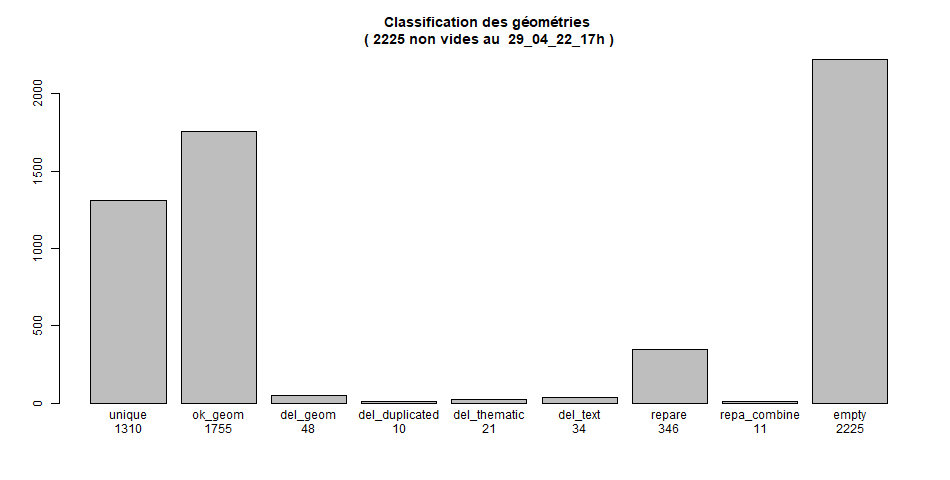
\includegraphics{./figures/bar_classify_Del_29_04_22_17h.png}

}

\caption{\label{fig-chart1}Chart Bar des NAS}

\end{figure}

Puis ci-dessous la Figure~\ref{fig-chart2} image lu avec \texttt{knit}
via un chunk r

\begin{figure}

{\centering 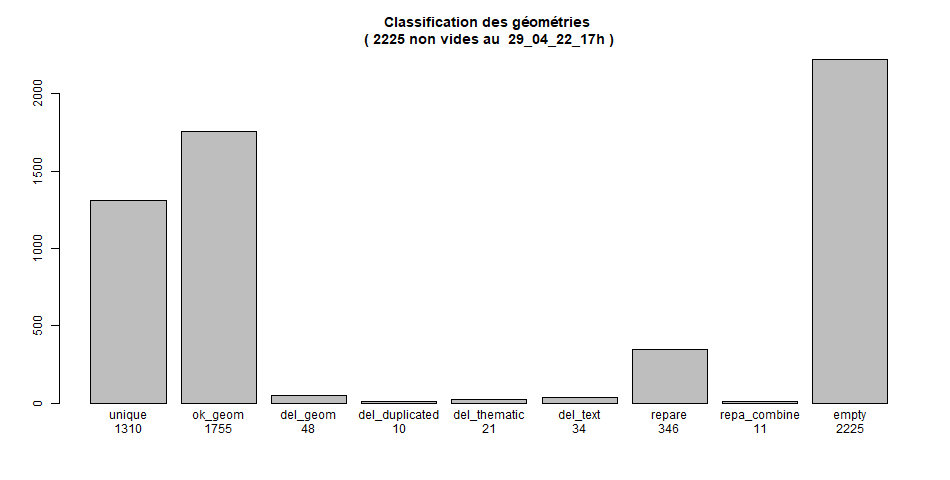
\includegraphics[width=3.17in,height=\textheight]{./figures/bar_classify_Del_29_04_22_17h.png}

}

\caption{\label{fig-chart2}Chart with Knitr}

\end{figure}

Voici le Figure~\ref{fig-chartCol} produit avec \texttt{R} et dont on ne
peut pas lire le (court) script et qui s'affiche sur deux colonnes

\begin{figure}

\begin{minipage}[t]{0.50\linewidth}

{\centering 

\raisebox{-\height}{

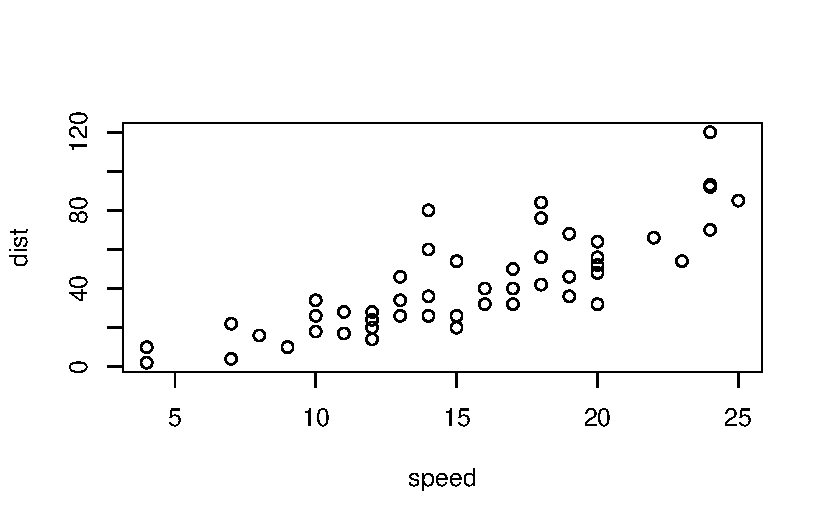
\includegraphics{./03_resultats_files/figure-pdf/fig-chartCol-1.pdf}

}

}

\subcaption{\label{fig-chartCol-1}Speed and Stopping Distances of Cars}
\end{minipage}%
%
\begin{minipage}[t]{0.50\linewidth}

{\centering 

\raisebox{-\height}{

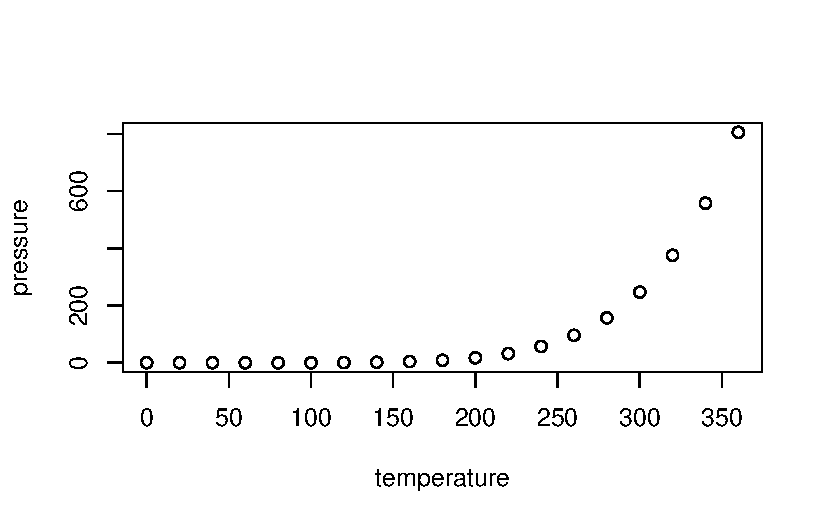
\includegraphics{./03_resultats_files/figure-pdf/fig-chartCol-2.pdf}

}

}

\subcaption{\label{fig-chartCol-2}Vapor Pressure of Mercury as a
Function of Temperature}
\end{minipage}%

\caption{\label{fig-chartCol}Two sided charts}

\end{figure}

Enfin la Figure~\ref{fig-plot-mtcars2} décrivant une courbe et son loess
ainsi que le script le construisant

\begin{Shaded}
\begin{Highlighting}[numbers=left,,]
\NormalTok{mtcars\_jj }\OtherTok{\textless{}{-}}\NormalTok{ mtcars}

\NormalTok{mtcars\_jj}\SpecialCharTok{$}\NormalTok{am }\OtherTok{\textless{}{-}} \FunctionTok{factor}\NormalTok{(}\AttributeTok{x =}\NormalTok{ mtcars}\SpecialCharTok{$}\NormalTok{am, }
                     \AttributeTok{labels =} \FunctionTok{c}\NormalTok{(}\StringTok{"automatic"}\NormalTok{, }\StringTok{"manuel"}\NormalTok{))}

\FunctionTok{ggplot}\NormalTok{(}\AttributeTok{data =}\NormalTok{ mtcars\_jj, }\FunctionTok{aes}\NormalTok{(hp, mpg, }\AttributeTok{color =}\NormalTok{ am)) }\SpecialCharTok{+}
  \FunctionTok{geom\_point}\NormalTok{() }\SpecialCharTok{+}
  \FunctionTok{geom\_smooth}\NormalTok{(}\AttributeTok{method =} \StringTok{"loess"}\NormalTok{) }\SpecialCharTok{+}
  \FunctionTok{theme}\NormalTok{(}\AttributeTok{legend.position =} \StringTok{"bottom"}\NormalTok{)}
\end{Highlighting}
\end{Shaded}

\begin{figure}[H]

{\centering 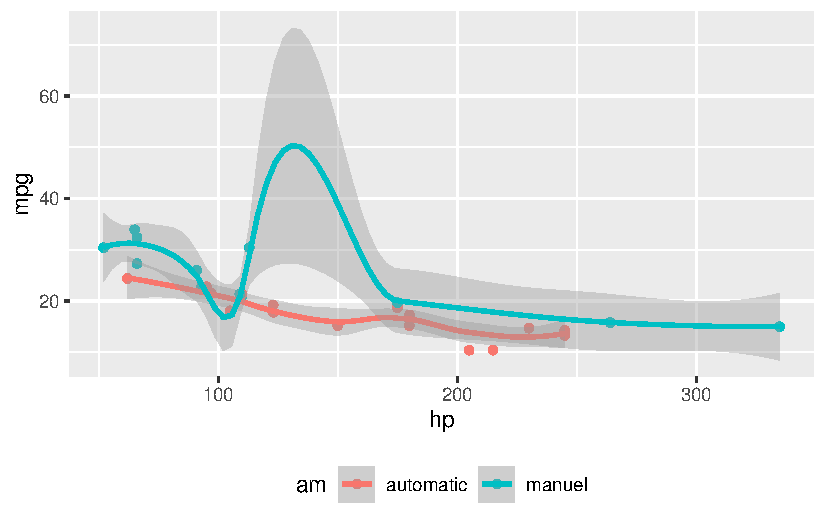
\includegraphics{./03_resultats_files/figure-pdf/fig-plot-mtcars2-1.pdf}

}

\caption{\label{fig-plot-mtcars2}MPG gorsepower}

\end{figure}

Ceci est un exemple de diagramme écrit en \texttt{mermaid}

\begin{Shaded}
\begin{Highlighting}[numbers=left,,]

\NormalTok{flowchart LR}
\NormalTok{  A[Hard edge] {-}{-}\textgreater{} B(Round edge)}
\NormalTok{  B {-}{-}\textgreater{} C\{Decision\}}
\NormalTok{  C {-}{-}\textgreater{} D[Result one]}
\NormalTok{  C {-}{-}\textgreater{} E[Result two]}
\end{Highlighting}
\end{Shaded}

\begin{figure}[H]

{\centering 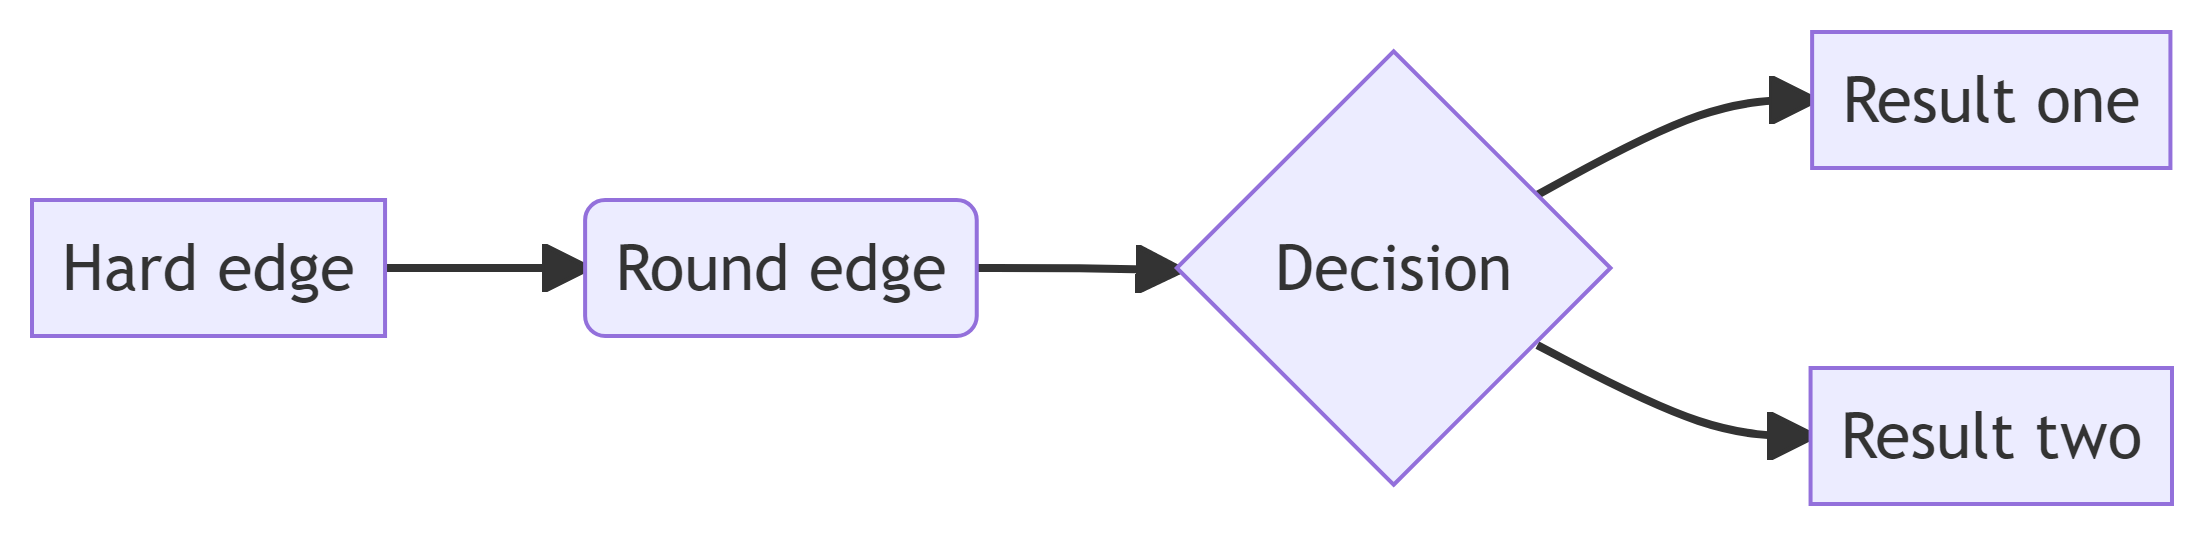
\includegraphics[width=5.74in,height=1.4in]{./03_resultats_files/figure-latex/mermaid-figure-1.png}

}

\end{figure}

Un autre exemple de diagramme

\begin{Shaded}
\begin{Highlighting}[numbers=left,,]

\NormalTok{sequenceDiagram}
\NormalTok{  participant Alice}
\NormalTok{  participant Bob}
\NormalTok{  Alice{-}\textgreater{}\textgreater{}John: Hello John, how are you?}
\NormalTok{  loop Healthcheck}
\NormalTok{    John{-}\textgreater{}\textgreater{}John: Fight against hypochondria}
\NormalTok{  end}
\NormalTok{  Note right of John: Rational thoughts \textless{}br/\textgreater{}prevail!}
\NormalTok{  John{-}{-}\textgreater{}\textgreater{}Alice: Great!}
\NormalTok{  John{-}\textgreater{}\textgreater{}Bob: How about you?}
\NormalTok{  Bob{-}{-}\textgreater{}\textgreater{}John: Jolly good!}
\end{Highlighting}
\end{Shaded}

\begin{figure}[H]

{\centering 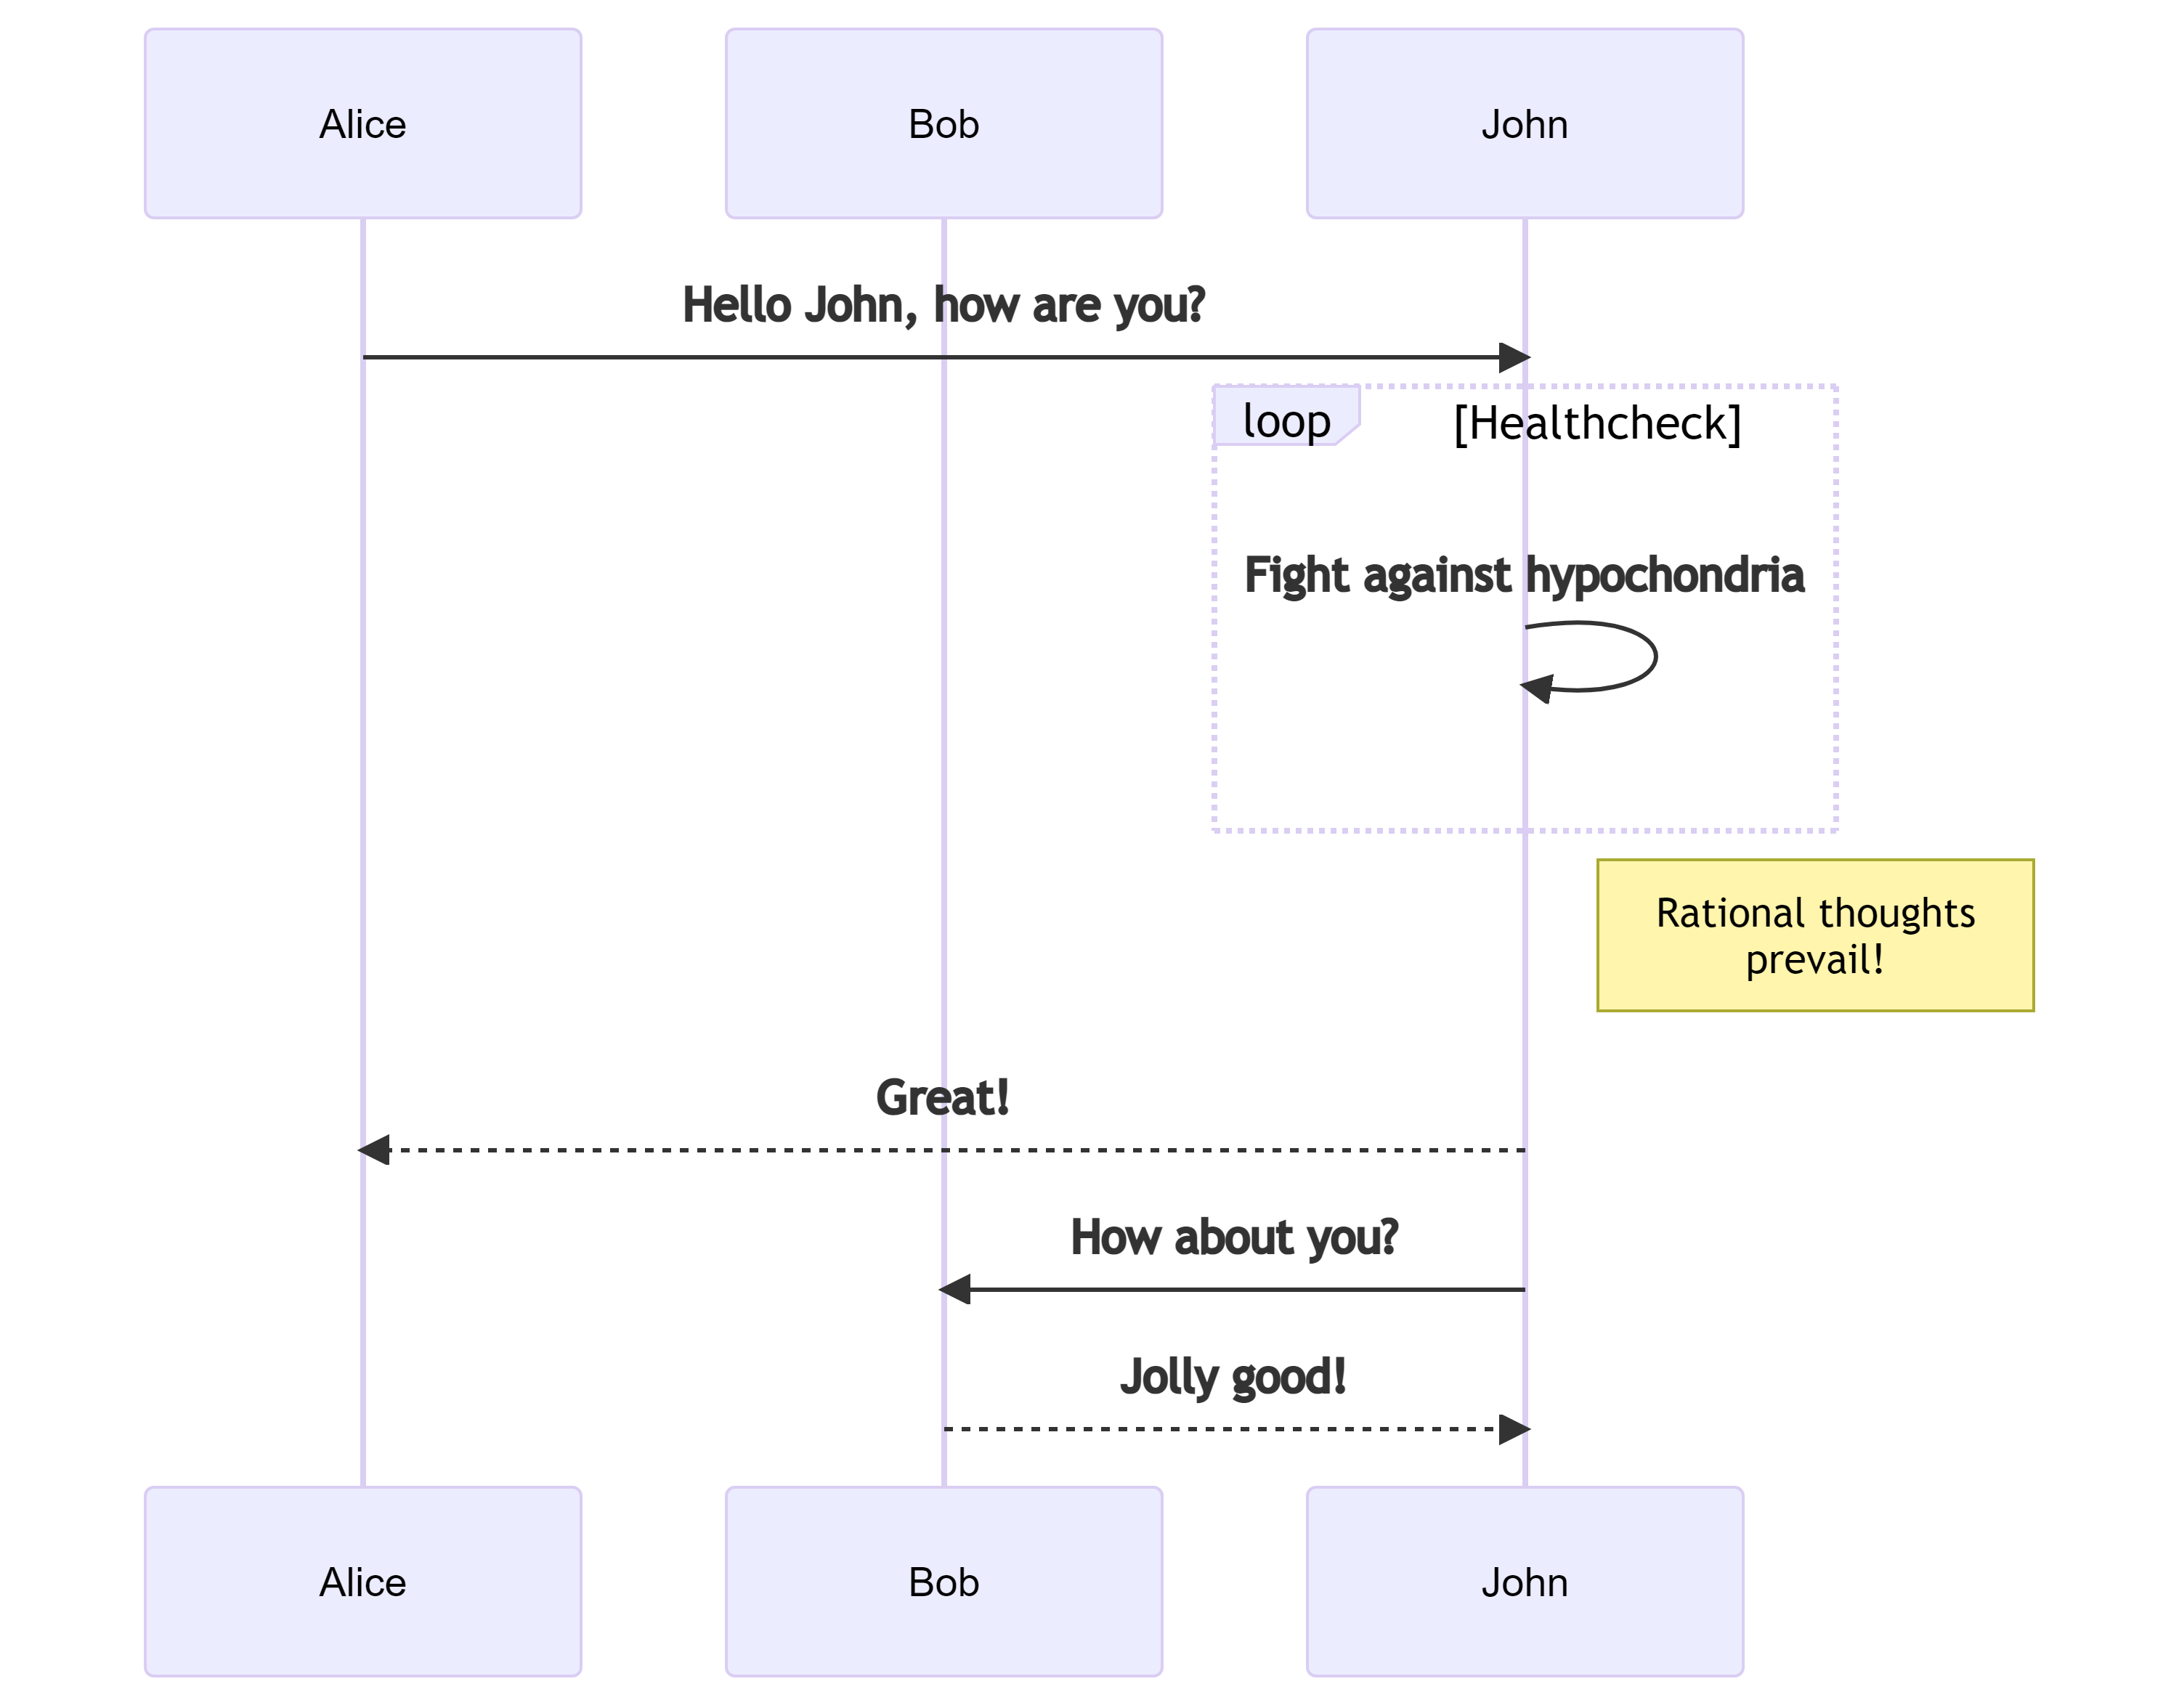
\includegraphics[width=7.81in,height=6.13in]{./03_resultats_files/figure-latex/mermaid-figure-2.png}

}

\end{figure}

mermaid diagram

\hypertarget{data}{%
\section{Data}\label{data}}

The penguins data from the
\href{https://allisonhorst.github.io/palmerpenguins}{\textbf{palmerpenguins}}
package contains size measurements for nrow(penguins) penguins from
three species observed on three islands in the Palmer Archipelago,
Antarctica.

The Figure~\ref{fig-plot-penguins} below shows the relationship between
flipper and bill lengths of these penguins.

\begin{Shaded}
\begin{Highlighting}[numbers=left,,]
\FunctionTok{ggplot}\NormalTok{(penguins, }
       \FunctionTok{aes}\NormalTok{(}\AttributeTok{x =}\NormalTok{ flipper\_length\_mm, }\AttributeTok{y =}\NormalTok{ bill\_length\_mm)) }\SpecialCharTok{+}
  \FunctionTok{geom\_point}\NormalTok{(}\FunctionTok{aes}\NormalTok{(}\AttributeTok{color =}\NormalTok{ species, }\AttributeTok{shape =}\NormalTok{ species)) }\SpecialCharTok{+}
  \FunctionTok{scale\_color\_manual}\NormalTok{(}\AttributeTok{values =} \FunctionTok{c}\NormalTok{(}\StringTok{"darkorange"}\NormalTok{,}\StringTok{"purple"}\NormalTok{,}\StringTok{"cyan4"}\NormalTok{)) }\SpecialCharTok{+}
  \FunctionTok{labs}\NormalTok{(}
    \AttributeTok{title =} \StringTok{"Flipper and bill length"}\NormalTok{,}
    \AttributeTok{subtitle =} \StringTok{"Dimensions for penguins at Palmer Station LTER"}\NormalTok{,}
    \AttributeTok{x =} \StringTok{"Flipper length (mm)"}\NormalTok{, }\AttributeTok{y =} \StringTok{"Bill length (mm)"}\NormalTok{,}
    \AttributeTok{color =} \StringTok{"Penguin species"}\NormalTok{, }\AttributeTok{shape =} \StringTok{"Penguin species"}
\NormalTok{  ) }\SpecialCharTok{+}
  \FunctionTok{theme\_minimal}\NormalTok{()}
\end{Highlighting}
\end{Shaded}

\begin{figure}[H]

{\centering 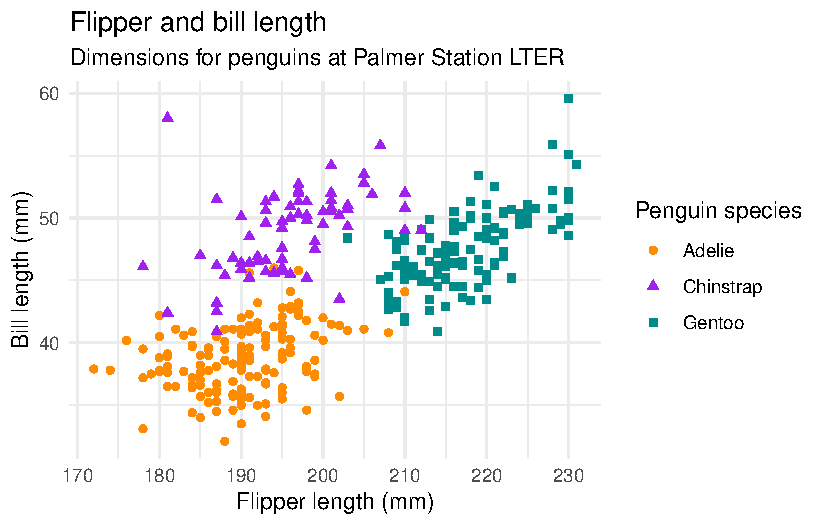
\includegraphics{./03_resultats_files/figure-pdf/fig-plot-penguins-1.pdf}

}

\caption{\label{fig-plot-penguins}Happy Penguins}

\end{figure}

\bookmarksetup{startatroot}

\hypertarget{conclusion}{%
\chapter*{Conclusion}\label{conclusion}}
\addcontentsline{toc}{chapter}{Conclusion}

Dans quelles conditions peut-on la généraliser ? Quelles réponses ont
été données ? Quelles sont celles qui ne l'ont pas été ? Que faut-il
envisager pour l'avenir ?

\bookmarksetup{startatroot}

\hypertarget{remerciements}{%
\chapter*{Remerciements}\label{remerciements}}
\addcontentsline{toc}{chapter}{Remerciements}

\bookmarksetup{startatroot}

\hypertarget{references}{%
\chapter*{References}\label{references}}
\addcontentsline{toc}{chapter}{References}

\hypertarget{refs}{}
\begin{CSLReferences}{1}{0}
\leavevmode\vadjust pre{\hypertarget{ref-bailly2005}{}}%
Bailly, Antoine. 2005. {``Voyage en Géographie.''} \emph{BSGLg},
January. \url{https://popups.uliege.be/0770-7576/index.php?id=1857}.

\leavevmode\vadjust pre{\hypertarget{ref-noucher2015}{}}%
Noucher, Matthieu. 2015. \emph{De la trace à la carte et de la carte à
la trace : pour une approche critique des nouvelles sources de fabrique
cartographique}. Presses des Mines.
\url{https://halshs.archives-ouvertes.fr/halshs-01212022}.

\end{CSLReferences}

\appendix
\addcontentsline{toc}{part}{Appendices}

\hypertarget{glossaire}{%
\chapter*{Glossaire}\label{glossaire}}
\addcontentsline{toc}{chapter}{Glossaire}

\hypertarget{quelques-ruxe9sultats-suppluxe9mentaires}{%
\chapter*{Quelques résultats
supplémentaires}\label{quelques-ruxe9sultats-suppluxe9mentaires}}
\addcontentsline{toc}{chapter}{Quelques résultats supplémentaires}

Some results that wouldn't fit into the main thesis

\begin{figure}

{\centering 
\includegraphics{./cover.png}

}

\caption{cover}

\end{figure}


\backmatter

\cleardoublepage
\newgeometry{margin=4cm}  
\pagestyle{empty}

\noindent
\textbf{\Large\MyTitle} \\

\noindent
\textbf{\textit{\MyAuthor}} \\
\noindent
\MyDate

\vspace{3mm}


\noindent
\rule{\textwidth}{0.7pt}


\vspace{5mm}

Résumé du stage (dont le sujet) en 10 lignes en français et en anglais. Informatif et concis, ce résumé doit refléter l'esprit du document, définir les buts et les méthodes, les résultats et les conclusions. Il se présente sous la forme d'un paragraphe unique, sans alinéa.



\vspace{10mm}


\noindent
\textbf{MOT CLEF}\\
\begin{itemize}
\item paradonnées
\item metadonnées
\item reproductibilité
\item base de donnée
\item géomatique
\item programmation lettrée
\end{itemize}



\begin{figure}[b]

\centerline{
\includegraphics[width=4in,height=1in]{figures/logos/logos3.jpg}}
\end{figure}



\clearpage

\restoregeometry












\end{document}
